% SC4051 --- Chapter 5: Replication (0->100)
\chapter{Replication: Primary-Backup, Quorums and Chains}
\label{ch:replication}

\begin{quote}
\emph{``Replication is the art of keeping copies close enough to be useful and far enough to survive.''} We want every read to see the right value, even when some copies are slow, stale or gone.
\end{quote}

\noindent\fbox{\parbox{\dimexpr\linewidth-2\fboxsep-2\fboxrule}{%
\textbf{From zero: why copy data and how to keep copies consistent.} We start with a single copy, add a second for availability, and discover the spectrum from eager to lazy replication. We then compare three families---primary-backup, quorum and chain---on consistency, latency and failure handling.}}
\vspace{0.4em}

\section*{Learning Outcomes}
After this chapter you will be able to:
\begin{enumerate}[label=(L\arabic*)]
    \item distinguish synchronous vs.\ asynchronous replication and state the data-loss window;
    \item describe primary-backup with log shipping and failover, including fencing;
    \item apply quorum replication ($R+W>N$) and tune $R,W$ for read/write trade-offs;
    \item explain chain replication and its linearizable, high-throughput pipeline;
    \item reason about replica consistency (read repair, anti-entropy, hinted handoff).
\end{enumerate}

% ============================================================
\section{Why Replicate?}
\label{sec:why-replicate}
Replication serves three goals: \emph{availability} (survive $f$ failures with $f+1$ copies, or $2f+1$ for strong consistency), \emph{durability} (geographic copies survive site failure), and \emph{performance} (nearby copy reduces latency, many copies increase read throughput). The price is consistency: writes must reach multiple copies, and the network between them is the bottleneck.

Two extremes frame the space. \emph{Eager (synchronous)} replication waits for replicas before acking the write---strong consistency, high latency, lower availability during partitions. \emph{Lazy (asynchronous)} replication acks after one copy and propagates in the background---low latency, higher availability, but reads may be stale and un-replicated writes can be lost on failover.

\begin{figure}[h]
\centering
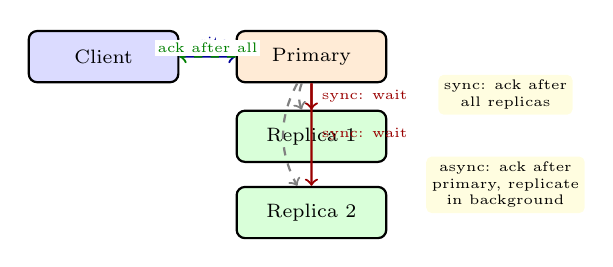
\begin{tikzpicture}[scale=0.88, every node/.style={font=\scriptsize},
  box/.style={draw,rounded corners=3pt,minimum width=1.9cm,minimum height=0.65cm,align=center,thick}]
\node[box,fill=blue!14] (cli) at (0,2.0) {Client};
\node[box,fill=orange!16] (pri) at (3.0,2.0) {Primary};
\node[box,fill=green!15] (rep1) at (3.0,0.85) {Replica 1};
\node[box,fill=green!15] (rep2) at (3.0,-0.25) {Replica 2};
\draw[->,thick,blue!60!black] (cli) -- (pri) node[midway,above,font=\tiny] {write};
\draw[->,thick,red!60!black] (pri) -- (rep1) node[midway,right,font=\tiny] {sync: wait};
\draw[->,thick,red!60!black] (pri) -- (rep2) node[midway,right,font=\tiny] {sync: wait};
\draw[->,thick,green!50!black,dashed] (pri) -- (cli) node[midway,above,font=\tiny,fill=white,inner sep=1pt] {ack after all};
% async hint
\node[font=\tiny,align=center,fill=yellow!12,rounded corners=2pt,inner sep=2pt] at (5.8,1.45) {sync: ack after\\all replicas};
\node[font=\tiny,align=center,fill=yellow!12,rounded corners=2pt,inner sep=2pt] at (5.8,0.15) {async: ack after\\primary, replicate\\in background};
\draw[->,thick,gray,dashed] (pri) to[bend right=20] (rep1);
\draw[->,thick,gray,dashed] (pri) to[bend right=28] (rep2);
\end{tikzpicture}
\caption{Synchronous vs.\ asynchronous replication. The dashed background arrows show async propagation that does not block the client ack.}
\label{fig:sync-async}
\end{figure}

% ============================================================
\section{Primary-Backup (Single-Leader)}
\label{sec:primary-backup}
One replica is the \emph{primary} (leader); all writes go through it. The primary orders writes, appends to its log, ships the log to backups, and acks after the chosen durability level (1 ack for async, majority for semi-sync, all for sync).

\paragraph{Failover.} When the primary fails, a backup is promoted. The hard problems are (i) \emph{detecting} failure without false positives (lease or heartbeat + timeout), (ii) \emph{fencing} the old primary so it cannot keep serving (STONITH, epoch/fencing token), and (iii) \emph{deciding} how much of the old primary's unreplicated tail to keep---discarding it loses acknowledged writes; keeping it needs consensus.

\begin{figure}[h]
\centering
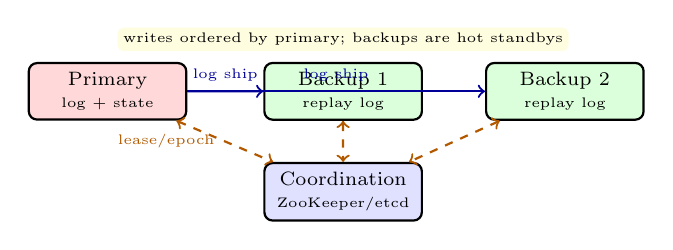
\begin{tikzpicture}[scale=0.88, every node/.style={font=\scriptsize},
  box/.style={draw,rounded corners=3pt,minimum width=2.0cm,minimum height=0.70cm,align=center,thick}]
\node[box,fill=red!15] (pri) at (0,1.6) {Primary\\{\tiny log + state}};
\node[box,fill=green!14] (b1) at (3.4,1.6) {Backup 1\\{\tiny replay log}};
\node[box,fill=green!14] (b2) at (6.6,1.6) {Backup 2\\{\tiny replay log}};
\node[box,fill=blue!12] (zk) at (3.4,0.15) {Coordination\\{\tiny ZooKeeper/etcd}};
\draw[->,thick,blue!60!black] (pri) -- (b1) node[midway,above,font=\tiny] {log ship};
\draw[->,thick,blue!60!black] (pri) -- (b2) node[midway,above,font=\tiny] {log ship};
\draw[<->,thick,orange!70!black,dashed] (pri) -- (zk) node[midway,left,font=\tiny] {lease/epoch};
\draw[<->,thick,orange!70!black,dashed] (b1) -- (zk);
\draw[<->,thick,orange!70!black,dashed] (b2) -- (zk);
\node[font=\tiny,fill=yellow!12,rounded corners=2pt,inner sep=2pt] at (3.4,2.35) {writes ordered by primary; backups are hot standbys};
\end{tikzpicture}
\caption{Primary-backup with log shipping. A coordination service holds the lease/epoch and fences the old primary on failover.}
\label{fig:primary-backup}
\end{figure}

\begin{lstlisting}[language=Python]
# Primary-backup: log shipping with fencing token (epoch)
class Primary:
    def __init__(self, epoch=1):
        self.epoch, self.log = epoch, []
        self.backups = []
    def add_backup(self, b): self.backups.append(b)
    def write(self, cmd):
        # fencing token (epoch) travels with every RPC so old primary is rejected
        self.log.append((self.epoch, cmd))
        acks = 1  # primary itself
        for b in self.backups:
            if b.replicate(self.epoch, self.log[-1]):
                acks += 1
        return acks

class Backup:
    def __init__(self): self.log, self.epoch = [], 0
    def replicate(self, epoch, entry):
        if epoch < self.epoch:   # fenced old primary
            return False
        self.epoch = epoch
        self.log.append(entry)
        return True

p, b1, b2 = Primary(epoch=3), Backup(), Backup()
p.add_backup(b1); p.add_backup(b2)
print("acks:", p.write("x:=10"))

# Failover: new primary with higher epoch fences old primary
p_new = Primary(epoch=4)
b1.epoch = 0  # simulate b1 accepting new primary
print("old primary after fencing:", p.write("y:=20"), " (b1 rejects if fenced)")
\end{lstlisting}

Without fencing, a network-partitioned old primary that still believes it is primary can serve stale writes---the classic \emph{split-brain}. Fencing tokens (monotonic epoch written to a coordination service) make the old primary's writes rejectable.

% ============================================================
\section{Quorum Replication}
\label{sec:quorum}
In \emph{quorum replication} (Gifford, 1979) there is no single primary. With $N$ replicas, a write contacts $W$ replicas and a read contacts $R$. If $R+W>N$, every read quorum overlaps every write quorum, so the read sees the latest write. Similarly $W+W>N$ ensures writes overlap (for compare-and-swap).

This gives tunable consistency:
\begin{equation}
R+W>N \;\land\; W > N/2 \quad\Longrightarrow\quad \text{strong (linearizable) with version numbers.}
\end{equation}
If $R+W\le N$, reads may be stale (eventual). Dynamo and Cassandra expose $R,W$ per operation so the same cluster can serve strong reads ($R=N,W=1$ is also overlapping but slow) or fast eventual reads ($R=1,W=1$).

\begin{figure}[h]
\centering
\begin{tikzpicture}[scale=0.88, every node/.style={font=\scriptsize}]
\foreach \i in {0,...,4} {
  \pgfmathsetmacro{\ang}{90 + \i*72}
  \node[draw,circle,fill=green!15,minimum size=0.85cm,thick] (n\i) at (\ang:1.6) {\tiny R\i};
}
\node[font=\tiny,fill=blue!12,rounded corners=2pt,inner sep=2pt] at (0,0) {$N=5$};
% write quorum W=3 highlighted
\begin{scope}[on background layer]
  \fill[red!12,rounded corners=4pt] (n0) -- (n1) -- (n4) -- cycle;
  \fill[blue!12,rounded corners=4pt] (n2) -- (n3) -- (n4) -- cycle;
\end{scope}
\node[font=\tiny,fill=red!12,rounded corners=2pt,inner sep=2pt] at (-2.4,0.55) {write $W=3$};
\node[font=\tiny,fill=blue!12,rounded corners=2pt,inner sep=2pt] at (2.4,0.55) {read $R=3$};
\node[font=\tiny,align=center] at (0,-2.15) {$R+W=6>5\Rightarrow$ overlap $\ge1$ node\\$R=3,W=3$ strong \quad $R=1,W=1$ eventual};
\end{tikzpicture}
\caption{Quorum overlap: with $N=5$, $R=3,W=3$ any read quorum meets any write quorum. Shrinking $R$ or $W$ trades consistency for latency.}
\label{fig:quorum}
\end{figure}

\paragraph{Repair.} Quorum reads may discover divergent versions. \emph{Read repair} pushes the newest version to stale replicas; \emph{anti-entropy} (Merkle trees, gossip) converges replicas in the background; \emph{hinted handoff} temporarily stores a write for a down replica on another node and replays when it returns.

\begin{lstlisting}[language=Python]
# Quorum replication simulation: R+W > N guarantees overlap
N, R, W = 5, 3, 3
replicas = {i: (0, None) for i in range(N)}  # (version, value)

def quorum_write(value, version, w_nodes):
    for n in w_nodes: replicas[n] = (version, value)

def quorum_read(r_nodes):
    # return value with highest version among read quorum
    best = max((replicas[n] for n in r_nodes), key=lambda x: x[0])
    # read-repair: push best to stale nodes in quorum
    for n in r_nodes:
        if replicas[n][0] < best[0]:
            replicas[n] = best
    return best

quorum_write("hello", version=1, w_nodes=[0,1,2])
print("read from [2,3,4]:", quorum_read([2,3,4]))  # must see version 1 via node 2
print("read from [3,4,0]:", quorum_read([3,4,0]))  # also sees it; repair heals 3,4
print("replicas:", replicas)
\end{lstlisting}

% ============================================================
\section{Chain Replication}
\label{sec:chain}
Chain replication (van Renesse--Schneider, 2004) arranges $N$ replicas in a chain. Writes enter at the \emph{head}, propagate through the chain, and are acked by the \emph{tail}. Reads go to the tail for strong consistency (or to any node for eventual).

The chain gives linearizable order without a separate consensus round per write: the chain \emph{is} the order. Throughput is high because nodes form a pipeline (head processes write $k+1$ while tail acks $k$). Failure handling needs a coordinator to splice out a failed node and re-chain.

Chain replication is the core of strongly consistent stores like CRAQ and of log systems where the chain maps to a replicated log.

\begin{example}[Chain read optimisation]
CRAQ (Chain Replication with Apportioned Queries) lets any chain node serve a \emph{dirty} read locally if it has seen the write, marking it dirty until the tail acknowledges. Clean reads go to the tail. This keeps strong consistency while spreading read load---useful when reads dominate writes by $10$--$100\times$.
\end{example}

\begin{remark}[Choosing a replication family]
Primary-backup is simplest when writes are naturally funnelled through one leader (single-key operations). Quorums shine for multi-key, leaderless workloads with tunable latency. Chains excel for log-structured, append-heavy stores where pipeline throughput matters. Many production stores combine them: e.g., a Paxos-replicated primary whose backups form a chain for log shipping.
\end{remark}

% ============================================================
\section{Exercises}
\label{sec:ch05-exercises}
\begin{enumerate}[label=E5.\arabic*, leftmargin=*, itemsep=0.6em]
    \item \textbf{Sync vs.\ async window.} A primary acks after the primary only (async) and ships to 2 backups with 10\,ms delay. If the primary crashes uniformly at random in a 1\,s window, what is the expected number of lost acknowledged writes at 100 writes/s? How does semi-sync ($W=2$) change the answer?
    \item \textbf{Fencing.} Without fencing, describe a split-brain scenario with a partitioned primary that keeps serving writes. Show how an epoch/fencing token stored in ZooKeeper prevents the old primary's writes from being accepted by backups after failover.
    \item \textbf{Quorum tuning.} With $N=5$, enumerate $(R,W)$ pairs for (a) strong consistency, (b) read-optimised strong, (c) write-optimised strong, (d) eventual. For each, state how many replica failures can be tolerated for reads and writes.
    \item \textbf{Chain vs.\ quorum.} Compare chain replication and quorum replication on (i) read latency, (ii) write throughput under pipeline, (iii) behaviour when the tail/head fails, (iv) load distribution. When would you prefer one over the other?
    \item \textbf{Anti-entropy.} Two replicas hold 1M keys each, differing in 10 keys. Explain why naive full comparison is wasteful and how Merkle trees let you find the differing keys in $O(\log n)$ exchanges. Sketch the tree walk.
\end{enumerate}

% ============================================================
\section*{Chapter Notes}
Gifford (1979) introduced weighted voting/quorums. Primary-backup and viewstamped replication: Oki--Liskov (1988). Chain replication: van Renesse--Schneider (OSDI, 2004); CRAQ: Terra--Shah (2009). Quorum tuning and Dynamo: DeCandia et al., ``Dynamo'' (SOSP, 2007). Fencing and leases: Kleppmann, Ch.~8--9. Anti-entropy and Merkle trees: Demers et al.\ (1987) and Dynamo's use of them.

% End of Chapter 5
